\documentclass[../report.tex]{subfiles}


\begin{document}

    \subsection{Gantt-Chart}
    A way to show the progress of the project is with a Gantt Chart. 
    In the following Gantt Chart it can be seen with the orange line, 
    when one part of the project started and ended. For example, for 
    choosing the components for the forklift it took from the 6/Oct/23
     until the 17/Oct/23, with a duration of 11 days.



 Figure : Gantt Chart of the time planning of the project Forklift

 \begin{figure}[h!]
    \centering
    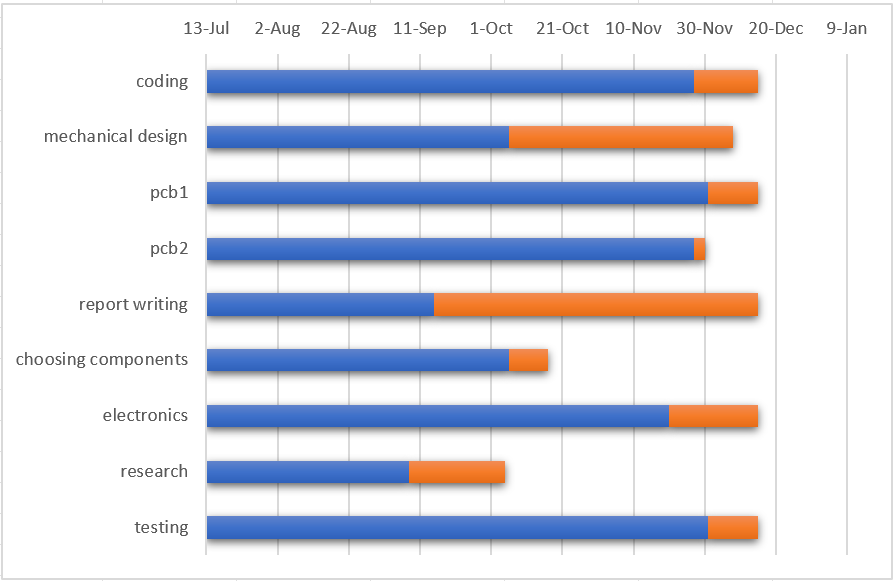
\includegraphics[width=1\textwidth]{gantt_chart_correct2.png}
    \caption{Gantt chart}
 \end{figure}
  
\end{document}

